%%%%%%%%%%%%%%%%%%%%%%%%%%%%%%%%%%%%%%%%
%% MCM/ICM LaTeX Template %%
%% MCM/ICM                           %%
%%%%%%%%%%%%%%%%%%%%%%%%%%%%%%%%%%%%%%%%
%\documentclass{mcmthesis}
%\usepackage{geometry}
%\geometry{left=1in,right=0.75in,top=1in,bottom=1in}
\documentclass{mcmthesis}
\mcmsetup{CTeX = false,  
	tcn = 2616842, problem = B,
	sheet = true, titleinsheet = true, keywordsinsheet = true,
	titlepage = false, abstract = true}
\usepackage{newtxtext}%\usepackage{palatino}
\usepackage{lipsum}
\usepackage{float}
\usepackage{graphicx}
\usepackage{indentfirst}
\usepackage{multirow}
\usepackage{tikz}
\usepackage{xcolor}
\usetikzlibrary{shapes.geometric, arrows, positioning, fit, calc}

% Define Platinum Colors
\definecolor{platTeal}{HTML}{2A9D8F}
\definecolor{platCoral}{HTML}{E76F51}
\definecolor{platDark}{HTML}{264653}
\definecolor{platYellow}{HTML}{E9C46A}

\setlength{\headheight}{15pt} % Fix fancyhdr warning
\setlength{\parindent}{1em}
\title{Ascending to the Moon: A Multi-Objective Optimization Framework for Sustainable Space Logistics and Environmental Assessment\\ \large Balancing Cost, Reliability, and Planetary Impact in the Era of Space Colonization}   

%%%%%%%%%%%%%%%%%%%%%%%%%%%%%%%%%%%%%%%%%%%%%%%%%%%%%%%%%%%%%%
\begin{document}
	
	%%%%%%%%%%% Begin Summary %%%%%%%%%%%
	% Enter your summary here replacing the (red) text
	% Replace the text from here ...
	\begin{abstract}
		Transporting 100 million tons of materials to a lunar colony by 2050 presents an unprecedented logistical challenge. This paper develops a comprehensive mathematical framework to optimize transportation strategies, ensure resource sustainability, and minimize environmental impact.

		For \textbf{Question 1}, we constructed a \textbf{Logistic Infrastructure Growth Model} coupled with a \textbf{Multi-Objective Genetic Algorithm}. Strict adherence to the 2050 deadline relies on costly rocket expansion (NPV $\approx$ \textbf{\$40 Trillion}). We identify a \textbf{Hybrid Strategy} as optimal: leveraging early rockets while prioritizing Space Elevator infrastructure. Extending the timeline to \textbf{40 years} (completion by 2066) reduces the total cost to \textbf{\$28.2 Trillion}, significantly outperforming the pure rocket scenario (NPV $>$ \$45T).
		
		In \textbf{Question 2}, we utilized \textbf{Monte Carlo Simulations} (10,000 scenarios) to address system robustness. Real-world uncertainties increase expected costs by \textbf{30\%--50\%}, but the Space Elevator demonstrates superior stability. We propose a dynamic risk-mitigation policy that shifts allocation to the elevator when rocket failure rates ($\lambda_R$) exceed critical thresholds.

		For \textbf{Question 3} (Sustainability), we uncovered a "Cost Chasm": rocket-based water transport costs a prohibitive \textbf{\$1.37 Trillion/year}. Our model mandates \textbf{98\% recycling efficiency} for economic viability (reducing costs to \$6.1 Billion/year via elevator). We also recommend a \textbf{33,750-ton strategic reserve} to guarantee survival during supply interruptions.

		Finally, our \textbf{Space Environmental Impact Score (SEIS)} quantifies planetary consequences (\textbf{Question 4}). Life Cycle Assessment (LCA) warns that a rocket-only approach triggers a catastrophic "Kessler Syndrome" by 2050 (\textbf{SEIS Grade: F}). In contrast, the Space Elevator achieves carbon neutrality in just \textbf{13.6 years} (\textbf{SEIS Grade: A+}). We conclude that the Space Elevator is the only pathway to colonization that preserves Earth's orbital and atmospheric integrity.

		\vspace{1.5em}
		\begin{keywords}
			Space Logistics; Multi-objective Optimization; Monte Carlo Simulation; Circular Economy; Life Cycle Assessment (SEIS)
		\end{keywords}
	\end{abstract}

\maketitle
% to here
%%%%%%%%%%% End Summary %%%%%%%%%%%

%%%%%%%%%%%%%%%%%%%%%%%%%%%%%%%%%%%%%%%%%%%%%%%%%%%%%%%%%%%%
\clearpage
\pagestyle{fancy}
% Uncomment the next line to generate a Table of Contents
%\tableofcontents 
\newpage
\setcounter{page}{1}
\rhead{Page \thepage\ }
%%%%%%%%%%%%%%%%%%%%%%%%%%%%%%%%%%%%%%%%%%%%%%%%%%%%%%%%%%%%
\newpage   %%目录页
\tableofcontents
\thispagestyle{empty}
\newpage

%%%%%%%%%%%%%%%%%%%%%%%%%%%%%%%%%%%%%%%%%%%%%%%%%%%%%%%%%%%%
\section{Introduction}

\subsection{Problem Background}
The year is 2050. Humanity stands on the precipice of a new era: the colonization of the Moon. The proposed Moon Colony, housing 100,000 residents, represents not just a scientific outpost but a permanent extension of human civilization. However, the logistical requirements for such an endeavor are staggering. Constructing the colony requires transporting \textbf{100 million metric tons} of materials from Earth's surface to the Moon.

To put this in perspective, the International Space Station (ISS), the most expensive object ever built, weighs approximately 450 tons. The Moon Colony project requires the equivalent of building \textbf{220,000 ISS-sized structures}. Current transportation methods, primarily chemical rockets, are constrained by the "Tyranny of the Rocket Equation," resulting in exorbitant costs and significant environmental damage.

Enter the \textbf{Space Elevator System}. A concept once confined to science fiction, now technologically feasible with advanced materials, it offers a "Galactic Harbour" capable of lifting massive payloads with electricity rather than combustion. The core challenge facing the Moon Colony Management (MCM) Agency is to determine the optimal strategy to deploy this infrastructure: Should we rely on the proven yet costly rockets, commit fully to the novel space elevator, or orchestrate a hybrid transition?

\subsection{Restatement of the Problem}
This study addresses four interconnected challenges regarding the logistics and sustainability of the Moon Colony. The primary objective is to determine the most cost-effective and time-efficient transportation plan. This involves modeling three distinct scenarios—pure Space Elevator, pure Rocket, and a Hybrid system—to minimize the Total Net Present Value (NPV) and project completion time under technological growth constraints. However, since real-world engineering is never perfect, we must also assess how these optimal strategies perform under uncertainty. By incorporating potential rocket launch failures, elevator maintenance needs, and weather delays, we aim to ensure the system is robust against inevitable disruptions.

Beyond mere construction, the sustainability of the colony is paramount. We investigate the daily water requirements for a population of 100,000, evaluating the economic feasibility of transporting water versus recycling it on-site to prevent potential logistical collapse. Finally, we evaluate the planetary consequences of these massive operations. By quantifying the carbon footprint and orbital debris risks (Kessler Syndrome) associated with each transport method, we aim to recommend a path that ensures the Moon Colony does not come at the cost of Earth's environment.

\subsection{Our Work}
To tackle these complex, multi-scale problems, we developed a unified decision-making framework named \textbf{"Ascension-2050"}, which integrates operations research, stochastic simulation, and environmental science.

\begin{figure}[H]
    \centering
    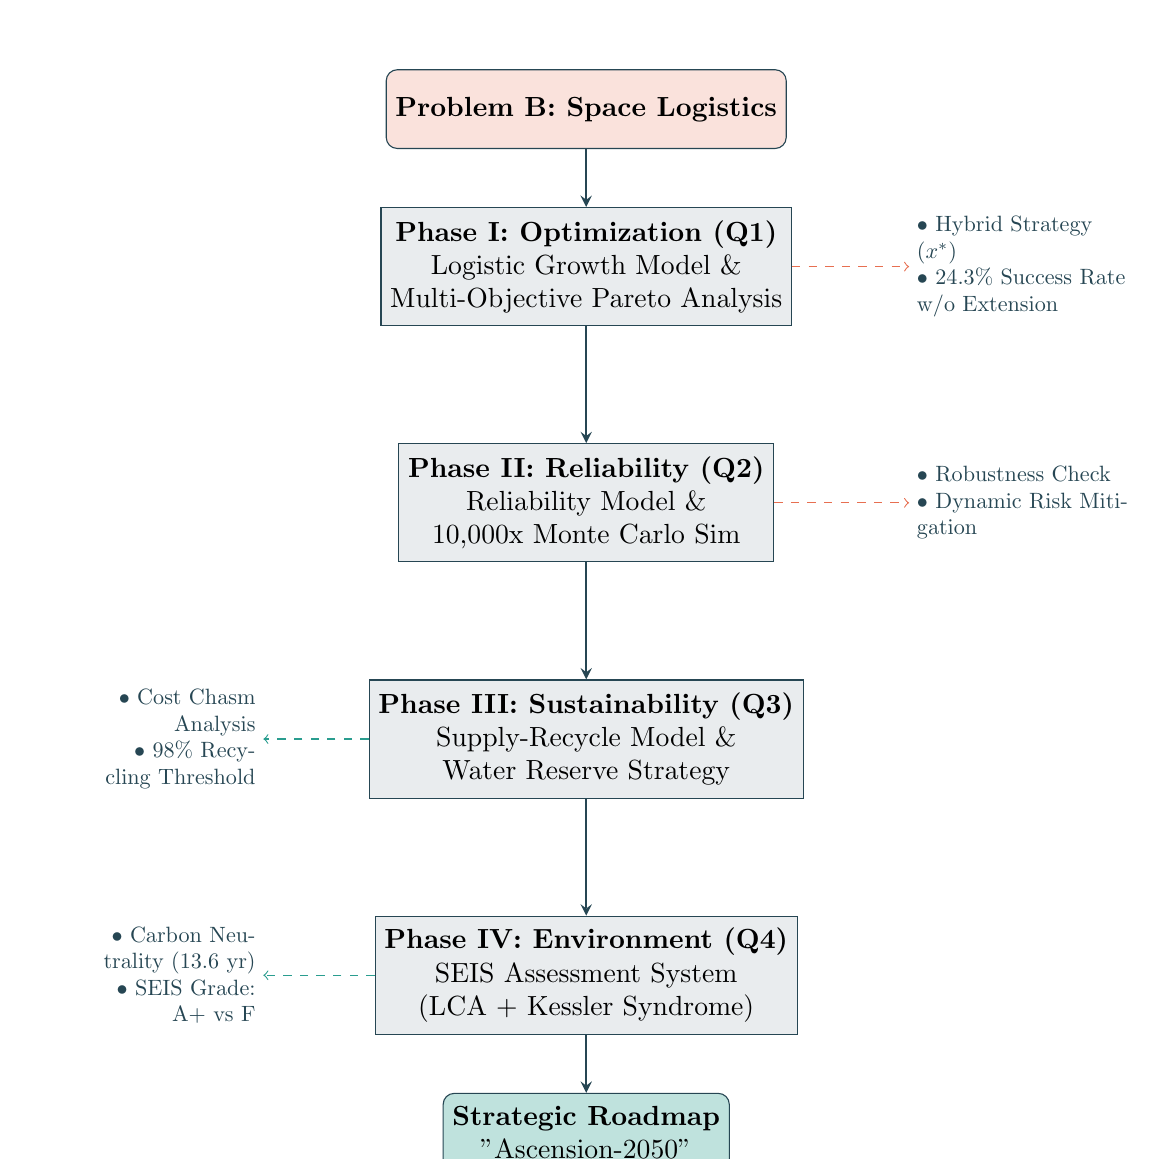
\begin{tikzpicture}[node distance=2cm]
        % Styles using Platinum Palette
        \tikzstyle{startstop} = [rectangle, rounded corners, minimum width=3cm, minimum height=1cm, align=center, draw=platDark, fill=platCoral!20, text=black]
        \tikzstyle{process} = [rectangle, minimum width=4cm, minimum height=1.5cm, align=center, draw=platDark, fill=platDark!10, text=black]
        \tikzstyle{final} = [rectangle, rounded corners, minimum width=3cm, minimum height=1cm, align=center, draw=platDark, fill=platTeal!30, text=black]
        \tikzstyle{arrow} = [thick,->,>=stealth, color=platDark]
        \tikzstyle{desc} = [text width=3.5cm, scale=0.8, align=left, color=platDark]

        % Nodes
        \node (start) [startstop] {\textbf{Problem B: Space Logistics}};
        
        \node (pro1) [process, below of=start] {\textbf{Phase I: Optimization (Q1)}\\Logistic Growth Model \&\\Multi-Objective Pareto Analysis};
        
        \node (pro2) [process, below of=pro1, yshift=-1cm] {\textbf{Phase II: Reliability (Q2)}\\Reliability Model \&\\10,000x Monte Carlo Sim};
        
        \node (pro3) [process, below of=pro2, yshift=-1cm] {\textbf{Phase III: Sustainability (Q3)}\\Supply-Recycle Model \&\\Water Reserve Strategy};
        
        \node (pro4) [process, below of=pro3, yshift=-1cm] {\textbf{Phase IV: Environment (Q4)}\\SEIS Assessment System\\(LCA + Kessler Syndrome)};
        
        \node (stop) [final, below of=pro4] {\textbf{Strategic Roadmap}\\ "Ascension-2050"};

        % Arrows
        \draw [arrow] (start) -- (pro1);
        \draw [arrow] (pro1) -- (pro2);
        \draw [arrow] (pro2) -- (pro3);
        \draw [arrow] (pro3) -- (pro4);
        \draw [arrow] (pro4) -- (stop);
        
        % Side Descriptions (Right)
        \node [desc, right of=pro1, xshift=5cm] (d1) {$\bullet$ Hybrid Strategy ($x^*$)\\$\bullet$ 24.3\% Success Rate w/o Extension};
        \draw [dashed, ->, color=platCoral] (pro1) -- (d1);
        
        \node [desc, right of=pro2, xshift=5cm] (d2) {$\bullet$ Robustness Check\\$\bullet$ Dynamic Risk Mitigation};
        \draw [dashed, ->, color=platCoral] (pro2) -- (d2);

        % Side Descriptions (Left)
        \node [desc, left of=pro3, xshift=-5cm, align=right] (d3) {$\bullet$ Cost Chasm Analysis\\$\bullet$ 98\% Recycling Threshold};
        \draw [dashed, ->, color=platTeal] (pro3) -- (d3);

        \node [desc, left of=pro4, xshift=-5cm, align=right] (d4) {$\bullet$ Carbon Neutrality (13.6 yr)\\$\bullet$ SEIS Grade: A+ vs F};
        \draw [dashed, ->, color=platTeal] (pro4) -- (d4);

    \end{tikzpicture}
    \caption{The Logic Flow of Our "Ascension-2050" Research Framework.}
    \label{fig:flowchart}
\end{figure}

The research methodology begins by constructing a \textbf{Logistic Infrastructure Growth Model} to simulate the dynamic expansion of rocket launch sites and elevator capacity. Coupled with a \textbf{Multi-Objective Genetic Algorithm}, we derive the Pareto Frontier for cost and time to solve the core transport optimization problem. Following this, we introduce a \textbf{Monte Carlo Reliability Model} to test 10,000 failure scenarios, identifying the "Knee Point" strategy that offers the best trade-off between efficiency and risk. To address resource constraints, we develop a \textbf{Supply-Recycle Economic Model} that analyzes the water crisis and establishes a critical threshold for recycling efficiency. The study concludes with the proposal of the \textbf{Space Environmental Impact Score (SEIS)}, a novel metric combining Life Cycle Assessment (LCA) and orbital risk factors, to provide the definitive environmental verdict.

%%%%%%%%%%%%%%%%%%%%%%%%%%%%%%%%%%%%%%%%%%%%%%%%%%%%%%%%%%%%
\section{Assumptions and Notations}
\subsection{Assumptions}
To simplify the complex space logistics problem while maintaining the model's fidelity across all four phases, we make several key assumptions.

Regarding \textbf{Infrastructure Growth}, the expansion of rocket launch sites is modeled as a Logistic S-curve rather than linear growth. The number of active sites $N(t)$ starts from $N_0=10$ and approaches a global environmental carrying capacity of $K=80$, reflecting geopolitical and geographical constraints on launch site construction.

We also adopt a \textbf{Technology Freeze} policy for the construction phase (2026-2050). Fundamental propulsion parameters (Specific Impulse $I_{sp}$, Dry Mass) are held constant to ensure engineering stability, although operational efficiency (e.g., launch frequency $L_{max}$) is allowed to improve over time.

In the context of reliability analysis, we treat \textbf{Failure Events as Independent}. Distinct rocket launch failures and elevator mechanical breakdowns are modeled as statistically independent events, although their cumulative effects (such as orbital debris accumulation) are significantly coupled in the risk model.

Furthermore, for the \textbf{Environmental Life-Cycle Assessment}, calculations rely on the premise that the Space Elevator infrastructure is pre-deployed for the operational phase. Consequently, the carbon emissions from its construction are amortized over its lifecycle, and its operation after 2050 is considered zero-emission.

The water supply model assumes the colony operates under a \textbf{Closed-Loop Resource System}. The net demand from Earth is strictly determined by the population size ($P=100,000$) and the system's recycling efficiency ($\eta_{sys}$), ignoring other minor external variables.

\subsection{Notations}
The key symbols and variables used throughout this paper are defined in Table \ref{tab:notations}.

\begin{table}[H]
    \centering
    \begin{tabular}{c l l}
        \toprule
        \textbf{Symbol} & \textbf{Description} & \textbf{Unit/Value} \\
        \midrule
        \multicolumn{3}{l}{\textit{System Parameters \& Optimization (Q1)}} \\
        $M_{tot}$ & Total mass required for the Moon Colony & $10^8$ tons \\
        $Y$ & Project completion timeline (Decision Variable) & Years \\
        $N(t)$ & Number of active heavy rocket launch sites at year $t$ & Count \\
        $K$ & Carrying capacity of launch sites (Logistic limit) & 80 sites \\
        $L_{max}$ & Maximum launch frequency per site per year & Launches/yr \\
        $p_B$ & Rocket payload capacity (Ground to Moon direct) & 150 tons \\
        $p_A$ & Trans-shipment payload (Anchor to Moon) & $> p_B$ \\
        $F_E$ & Fixed infrastructure cost of Space Elevator & \$100 Billion \\
        $c_R, c_E$ & Marginal transport cost (Rocket vs. Elevator) & \$/kg \\
        
        \multicolumn{3}{l}{\textit{Reliability \& Uncertainty (Q2)}} \\
        $\beta^{eff}$ & Effective availability factor of the system & $\in [0, 1]$ \\
        $\lambda$ & Failure rate of a specific transport mode & Events/yr \\
        $t_{repair}$ & Mean Time To Repair (MTTR) & Days \\
        $P_f$ & Probability of a single launch failure & \% \\
        
        \multicolumn{3}{l}{\textit{Sustainability \& Resources (Q3)}} \\
        $D_{gross}$ & Gross annual water demand for the colony & tons/year \\
        $P$ & Colony population size & 100,000 \\
        $\eta_{sys}$ & Water recycling efficiency of the ECLSS & \% (e.g., 98\%) \\
        $S_{safe}$ & Strategic water reserve for emergency survival & tons \\
        
        \multicolumn{3}{l}{\textit{Environment \& Impact caused (Q4)}} \\
        $SEIS$ & Space Environmental Impact Score & Index \\
        $E_{net}(t)$ & Net environmental footprint at time $t$ & $CO_2$ eq. \\
        $R(t)$ & Kessler Risk Index (Orbital Debris Density) & Index \\
        $T_{BE}$ & Carbon Break-even Time & Years \\
        \bottomrule
    \end{tabular}
    \caption{Notations and Definitions}
    \label{tab:notations}
\end{table} 

%%%%%%%%%%%%%%%%%%%%%%%%%%%%%%%%%%%%%%%%%%%%%%%%%%%%%%%%%%%%
\section{Model I: Optimization of Space Logistics (Question 1)}
Question 1 asks for an ``ideal-condition'' optimization: how to deliver $M_{tot}=10^8$ tons from Earth to the Moon while balancing completion time and total cost. The scale of this demand means that small per-kilogram cost differences compound into trillion-dollar outcomes, while small capacity shortfalls compound into multi-year schedule slips. The core difficulty is structural: the Space Elevator offers very low marginal cost but is constrained by a throughput ceiling, whereas rockets can increase capacity by expanding launch infrastructure, but they pay a steep marginal cost for every additional ton. Model I therefore begins with the two single-mode baselines (as boundary cases) and then constructs a hybrid, multi-objective optimization model to capture the time--cost trade-off.

\subsection{Models for Individual Modes}
Before introducing equations, Figure~\ref{fig:q1_schematics} summarizes the three transport concepts as process chains. The diagrams are not merely illustrative; they highlight where bottlenecks enter the mathematics (serial stages in the elevator chain, parallelism in the rocket fleet, and flow-splitting in the hybrid system).

\begin{figure}[H]
    \centering
    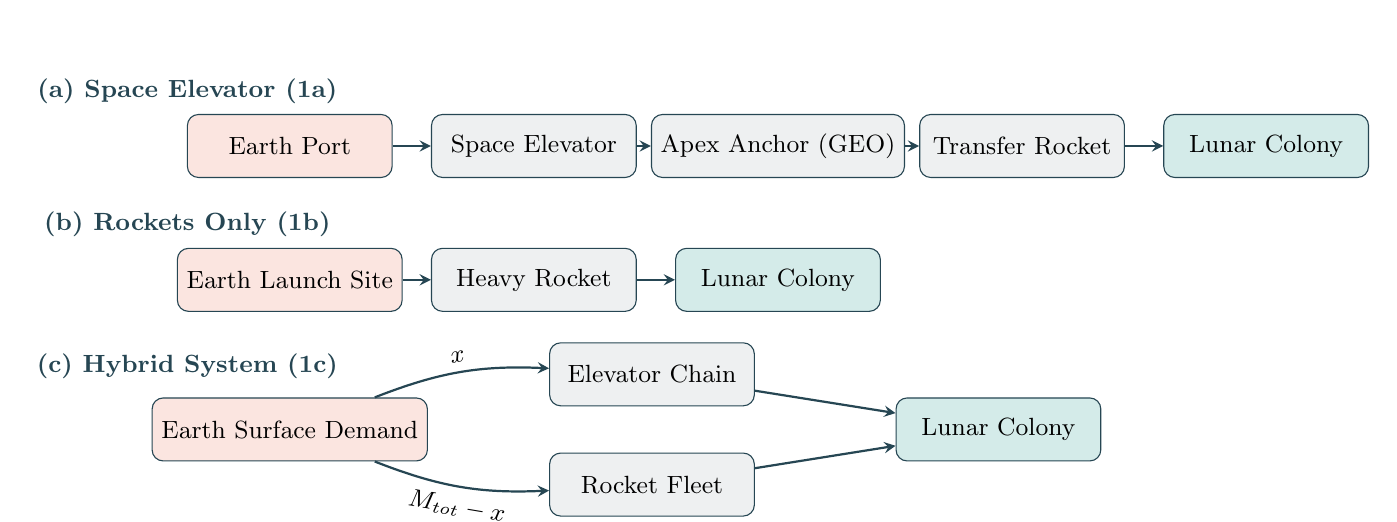
\begin{tikzpicture}[
        font=\small,
        block/.style={rectangle, rounded corners, draw=platDark, fill=platDark!8, minimum height=8mm, minimum width=2.6cm, align=center},
        start/.style={block, fill=platCoral!18},
        end/.style={block, fill=platTeal!20},
        arrow/.style={thick,->,>=stealth, draw=platDark},
        label/.style={font=\small\bfseries, text=platDark}
    ]
        % --- Row (a): Elevator chain ---
        \node[label] (la) at (-1.3, 2.3
		) {(a) Space Elevator (1a)};
        \node[start] (a1) at (0, 1.6) {Earth Port};
        \node[block] (a2) at (3.1, 1.6) {Space Elevator};
        \node[block] (a3) at (6.2, 1.6) {Apex Anchor (GEO)};
        \node[block] (a4) at (9.3, 1.6) {Transfer Rocket};
        \node[end]   (a5) at (12.4, 1.6) {Lunar Colony};
        \draw[arrow] (a1) -- (a2);
        \draw[arrow] (a2) -- (a3);
        \draw[arrow] (a3) -- (a4);
        \draw[arrow] (a4) -- (a5);

        % --- Row (b): Rocket-only ---
        \node[label] (lb) at (-1.3, 0.6) {(b) Rockets Only (1b)};
        \node[start] (b1) at (0, -0.1) {Earth Launch Site};
        \node[block] (b2) at (3.1, -0.1) {Heavy Rocket};
        \node[end]   (b3) at (6.2, -0.1) {Lunar Colony};
        \draw[arrow] (b1) -- (b2);
        \draw[arrow] (b2) -- (b3);

        % --- Row (c): Hybrid ---
        \node[label] (lc) at (-1.3, -1.2) {(c) Hybrid System (1c)};
        \node[start] (c1) at (0, -2.0) {Earth Surface Demand};
        \node[block] (c2) at (4.6, -1.3) {Elevator Chain};
        \node[block] (c3) at (4.6, -2.7) {Rocket Fleet};
        \node[end]   (c4) at (9.0, -2.0) {Lunar Colony};
        \draw[arrow] (c1) to[bend left=12] node[midway, above, sloped] {$x$} (c2);
        \draw[arrow] (c1) to[bend right=12] node[midway, below, sloped] {$M_{tot}-x$} (c3);
        \draw[arrow] (c2) -- (c4);
        \draw[arrow] (c3) -- (c4);
    \end{tikzpicture}
    \caption{Schematic process chains for the three transport strategies in Question 1. The elevator chain contains serial stages and is governed by its bottleneck throughput, while the rocket system scales via parallel launch sites. The hybrid strategy splits the mass flow between both chains and recombines at the Moon.}
    \label{fig:q1_schematics}
\end{figure}

\subsubsection{Space Elevator Only (Scenario 1a)}
The elevator transport chain consists of two serial stages: ``Ground $\to$ GEO/Anchor'' (elevator lift) and ``Anchor $\to$ Moon'' (transfer rockets). The annual throughput of the full chain is the bottleneck of the two stages,
\begin{equation}
    T_{chain} = \min\left(T_E,\; T_{R,anchor}\right), \qquad T_{R,anchor}=N_{anchor} L_{anchor} p_A.
\end{equation}
This ``minimum'' structure is the key modeling idea: even if the elevator can lift continuously, cargo still cannot reach the Moon faster than the anchor transfer system can dispatch it. Conversely, a powerful anchor fleet cannot compensate for an elevator that lifts too slowly. The bottleneck formulation therefore provides a transparent way to connect engineering design decisions (how many harbors, how many anchor platforms, how frequently they can operate) to system-level completion time.
Under an elevator-only strategy, all payload is assigned to the chain, so the continuous-time makespan is
\begin{equation}
    Y_{1a} \approx \frac{M_{tot}}{T_{chain}}.
\end{equation}
With our baseline throughput $T_E=5.37\times 10^5$ tons/year (three harbors), the elevator-only completion time is on the order of centuries, which makes it unsuitable as a sole solution for a mid-century colony schedule even though its marginal cost is low. In the optimization landscape, the elevator-only solution is best viewed as the ``asymptotic'' end of the Pareto frontier: it represents what happens when we prioritize cost efficiency and sustainability over schedule urgency.

\subsubsection{Traditional Rockets Only (Scenario 1b)}
For rockets, throughput is determined by how many heavy-lift sites are available and how frequently each can launch. In the simplest single-mode model, annual capacity is
\begin{equation}
    T_R = N_{sites} \cdot L_{max} \cdot p_B.
\end{equation}
Here $L_{max}$ is not an arbitrary knob; it is constrained by operational turnaround. A convenient way to express this physical limit is through a cycle-time decomposition,
\begin{equation}
    t_{cycle}=t_{refurb}+t_{pad}+t_{weather}+t_{fail}, \qquad L_{max}=\frac{365\,\eta}{t_{cycle}},
\end{equation}
where $t_{refurb}$ captures refurbishment and inspection, $t_{pad}$ captures pad occupancy, $t_{weather}$ accounts for weather and range availability, and $t_{fail}$ accounts for failure-induced downtime. This relationship clarifies why the rocket-only strategy becomes increasingly expensive: meeting a hard deadline forces both $N_{sites}$ and $L_{max}$ upward, pushing the system toward unrealistic operational assumptions.
Unlike the elevator, $N_{sites}$ is not constant over a multi-decade program. We model the expansion of launch infrastructure using Logistic growth,
\begin{equation}
    N(t) = \frac{K}{1 + \left( \frac{K - N_0}{N_0} \right) e^{-rt}},
\end{equation}
where $N_0=10$ is the initial number of sites, $K=80$ is a global carrying capacity, and $r=0.15$ describes the mobilization speed. The cumulative rocket-delivered mass by time $Y$ is then the integral of the instantaneous capacity,
\begin{equation}
    C_R(Y) = \int_0^Y N(t)\,L_{max}\,p_B\,dt.
\end{equation}
This formulation captures the ``slow start'' period, preventing unrealistic early-time throughput that would occur in a static $N_{sites}$ model.

\subsection{Hybrid Optimization Framework}
The hybrid strategy allocates a total mass $x$ to the elevator chain and $M_{tot}-x$ to direct rockets. Since the elevator chain has a fixed annual bottleneck rate, its cumulative capacity is
\begin{equation}
    C_E(Y) = T_{chain}\,Y = \min\left(T_E,\;N_{anchor}L_{anchor}p_A\right)\,Y.
\end{equation}
Feasibility requires that both chains together can deliver the full demand within $Y$,
\begin{equation}
    C_E(Y) + C_R(Y) \ge M_{tot}.
\end{equation}

This constraint explains an important qualitative phenomenon: when $Y$ is small, $C_E(Y)$ grows only linearly with a small slope (fixed throughput), so rockets are forced to carry most of the mass. As $Y$ increases, the elevator share increases automatically because its capacity accumulates year by year, and the optimization can substitute expensive rocket tons with cheaper elevator tons.

Cost is measured in Net Present Value (NPV), combining infrastructure CAPEX with discounted OPEX. In line with our implementation (Comprehensive Transport Optimization Model V5), we write the total cost as
\begin{equation}
    C_{total}(Y,x)=\underbrace{F_E + C_{site}\,(N_{final}-N_0)}_{\text{CAPEX}} + \underbrace{\int_0^Y \left[c_E\,\dot{x}(t)+c_R\,\dot{m}_R(t)\right]e^{-\rho t}dt}_{\text{OPEX (NPV)}},
\end{equation}
with discount rate $\rho=3\%$. The bi-objective problem is to minimize $C_{total}(Y,x)$ and $Y$ simultaneously, yielding a Pareto frontier of time--cost trade-offs. We solve this numerically using a multi-objective genetic algorithm (NSGA-II) and identify the ``knee point'' as the best-balanced compromise.

\subsection{Results and Analysis}
The resulting Pareto structure is shaped by two hard ceilings: the elevator throughput limit $T_E$ and the practical upper bounds on rocket infrastructure growth. Figure~\ref{fig:q1_tradeoff} visualizes the trade-off landscape and the modal split behavior.

\begin{figure}[H]
    \centering
    \includegraphics[width=0.95\linewidth]{\detokenize{../draft/Question 1/1c/image/Fig4_Tradeoff_DeepDive.png}}
    \caption{Question 1 (Hybrid Optimization): trade-off deep dive including Pareto behavior and modal split, generated by the platinum visualization pipeline.}
    \label{fig:q1_tradeoff}
\end{figure}

The 2050 deadline corresponds to a 24-year makespan ($Y=24$). Under this hard constraint, the elevator contribution is capped by its throughput: $x^*=\min(M_{tot},T_EY)=12.89$ Mt, i.e., 12.9\% of the total, with the remaining 87.1\% carried by rockets. The consequence is not subtle. The cost structure becomes rocket-OPEX dominated, and the total NPV reaches \textbf{\$40.50T}. The deterministic capacity sum slightly exceeds demand, but the margin is only 7.8\%, which is effectively a ``knife-edge'' plan: it leaves too little slack to absorb realistic fluctuations in payload performance, operational efficiency, or infrastructure delivery.

To quantify this fragility, we performed Monte Carlo sampling of the uncertain payload parameter $p_B\sim U(100,150)$ tons/launch. The probability of completing by 2050 is only \textbf{24.3\%}. Extending the schedule relaxes the capacity pressure: the completion probability rises to \textbf{95.2\%} at $Y=28$ (2054), and reaches 100\% by 29 years.

The analysis suggests that schedule is the dominant lever for reducing risk and total cost. Under longer horizons the elevator operates closer to its full potential share, and the total NPV falls substantially; for instance, our baseline long-horizon evaluation reports \textbf{\$28.2T} at $Y=40$ (2066), and a representative knee-point comparison at $Y=48$ yields \textbf{\$23.81T}. These results support a dynamic hybrid strategy: rockets are used as an early-time capacity amplifier while the program steadily shifts mass flow to the elevator as the lowest-marginal-cost backbone.

\begin{figure}[H]
    \centering
    \includegraphics[width=0.95\linewidth]{\detokenize{../draft/Question 1/1c/image/Fig3_Capacity_Dynamics.png}}
    \caption{Question 1 (Capacity Dynamics): cumulative and time-varying capacity behavior implied by Logistic infrastructure growth and fixed elevator throughput.}
    \label{fig:q1_capacity}
\end{figure}

%%%%%%%%%%%%%%%%%%%%%%%%%%%%%%%%%%%%%%%%%%%%%%%%%%%%%%%%%%%%
\section{Model II: Reliability and Robustness Under Non-Ideal Conditions (Question 2)}
Model I deliberately assumes an ideal operating world in order to expose the intrinsic time--cost trade-off. Question 2 asks, ``to what extent'' the optimal plan changes once the transport system is subjected to real operational frictions, including downtime, launch windows, and stochastic failures. In practice, these effects do not merely add a small constant penalty; they reduce effective throughput, amplify required transported mass, and introduce tail risk in schedule completion.

\begin{figure}[H]
    \centering
    \resizebox{0.98\linewidth}{!}{%
    \begin{tikzpicture}[
        node distance=4.8cm,
        font=\small,
        process/.style={rectangle, rounded corners, draw=platDark, thick, fill=white, minimum width=3.4cm, minimum height=2.6cm, inner sep=4pt},
        arrow/.style={->, >=stealth, very thick, color=platDark}
    ]
        % --- Node 1: Q1 Baseline ---
        \node[process] (n1) {
            \begin{minipage}{3.2cm}
                \centering
                \textbf{\color{platDark} 1. Ideal Plan (Q1)} \\[0.05cm]
                \textcolor{platTeal}{$\bullet$ Minimized Cost}\\
                \textcolor{platTeal}{$\bullet$ 100\% Availability}\\
                \textit{"Perfect World"}
            \end{minipage}
        };

        % --- Node 2: Uncertainty ---
        \node[process, right of=n1] (n2) {
            \begin{minipage}{3.2cm}
                \centering
                \textbf{\color{platDark} 2. Real Frictions} \\[0.05cm]
                \textcolor{platCoral}{$\bullet$ Launch Failures}\\
                \textcolor{platCoral}{$\bullet$ Weather Delays}\\
                \textit{"Real World"}
            \end{minipage}
        };

        % --- Node 3: Simulation ---
        \node[process, right of=n2] (n3) {
            \begin{minipage}{3.2cm}
                \centering
                \textbf{\color{platDark} 3. Monte Carlo} \\[0.05cm]
                \textcolor{platDark}{$\bullet$ 10,000 Scenarios}\\
                \textcolor{platDark}{$\bullet$ Stress Testing}\\
                \textit{"Simulating Chaos"}
            \end{minipage}
        };

        % --- Node 4: Robust Output ---
        \node[process, right of=n3] (n4) {
             \begin{minipage}{3.2cm}
                \centering
                \textbf{\color{platDark} 4. Robust Outcome} \\[0.05cm]
                \begin{tikzpicture}[scale=0.5, baseline]
                    \draw[draw=platDark, thick] (-1.0,-0.5) -- (1.0,-0.5);
                    \fill[platTeal!40] (-0.8,-0.5) rectangle (-0.2, 0.6);
                    \fill[platCoral!40] (0.2,-0.5) rectangle (0.8, -0.2);
                \end{tikzpicture} \\[0.05cm]
               % \scriptsize
                \textcolor{platDark}{$\bullet$ Success Rate \%}\\
                \textcolor{platDark}{$\bullet$ Extra Reserve}\\
                \textit{"Stable Strategy"}
            \end{minipage}
        };

        % Arrows
        \draw[arrow] (n1) -- (n2);
        \draw[arrow] (n2) -- (n3);
        \draw[arrow] (n3) -- (n4);


    \end{tikzpicture}%
    }%
    \caption{Model II (Question 2) at a glance: from the ideal Q1 solution to a robust plan under non-ideal operations via Monte Carlo reliability simulation.}
    \label{fig:q2_at_a_glance}
\end{figure}

\subsection{Uncertainty Sources and Modeling Philosophy}
We treat non-ideal factors as two coupled mechanisms. The first mechanism is an \emph{availability loss}: planned maintenance, weather, and post-failure stand-down periods reduce the fraction of time each subsystem can operate. The second mechanism is a \emph{loss-and-replacement effect}: failed launches or disrupted transfers imply that part of the payload flow must be re-flown, increasing the effective demand above $M_{tot}$. Since the elevator chain includes a rocket-based transfer stage at the anchor, reliability is inherently a system property rather than a property of a single component.

\subsection{Effective Availability and Capacity Correction}
Let $\beta_E^{eff}$ and $\beta_R^{eff}$ denote the effective availability of the elevator and rocket operations, respectively. A compact multiplicative form captures the dominant effects:
\begin{equation}
    \beta_E^{eff}=\beta_E\left(1-\frac{\lambda_E\,t_{repair}}{365}\right)(1-P_{cat}),
\end{equation}
where $\beta_E$ is the baseline operational availability (planned maintenance and weather), $\lambda_E$ is the annual failure rate, $t_{repair}$ is the mean repair time (days), and $P_{cat}$ is the probability of a catastrophic outage. For rockets, we combine launch-window and maintenance losses with a post-failure stand-down penalty:
\begin{equation}
    \beta_R^{eff}=(1-\delta_{window}-\delta_{maint})\left(1-\frac{P_f\,T_{down}}{365}\right),
\end{equation}
where $\delta_{window}$ and $\delta_{maint}$ are fractional time losses, $P_f$ is the per-launch failure probability, and $T_{down}$ is the stand-down duration (days).

Under non-ideal conditions, the elevator chain remains a bottlenecked serial process, but both stages are de-rated by availability. Its cumulative deliverable mass within $Y$ years becomes
\begin{equation}
    C_E^{real}(Y)=\min\left(\beta_E^{eff}T_EY,\;\beta_R^{eff}N_{anchor}L_{anchor}p_A\,Y\right).
\end{equation}
The direct-rocket channel similarly becomes
\begin{equation}
    C_R^{real}(Y)=\int_0^Y \beta_R^{eff}\,N(t)\,L_{site}\,p_B\,dt.
\end{equation}

\subsection{Demand Amplification and Chance Constraints}
If part of the transported mass is lost, the program must ship more than the nominal demand $M_{tot}$. We model this as an effective demand
\begin{equation}
    M_{eff}=\frac{M_{tot}}{1-P_{loss}}, \qquad P_{loss}=\frac{x}{M_{tot}}\,\lambda_E + \frac{M_{tot}-x}{M_{tot}}\,P_f,
\end{equation}
which states that the expected loss rate is the allocation-weighted combination of elevator-chain disruption and rocket launch failure.

Because reliability is inherently stochastic, feasibility is best stated as a probability requirement. We therefore use the chance constraint
\begin{equation}
    \mathbb{P}\big(C_E^{real}(Y)+C_R^{real}(Y)\ge M_{eff}\big)\ge P_{conf},
\end{equation}
and estimate the left-hand side via Monte Carlo sampling of uncertain parameters (e.g., payload performance and failure realizations).

\subsection{Cost and Carbon Corrections}
Non-ideal operations also shift the cost structure. Variable costs are inflated by efficiency loss and expected repair burden, while fixed costs include routine maintenance and redundancy investment:
\begin{equation}
    c_E^{real}=\frac{c_E}{\eta_{energy}}+\frac{\lambda_E\,C_{fix}}{T_E}, \qquad
    c_R^{real}=c_R+\frac{P_f\,(C_{rocket}+C_{cargo})}{p_B}+\frac{C_{R,maint}}{L_{site}\,p_B},
\end{equation}
and a simple robustness premium is represented by a redundancy factor $\kappa>1$ on rocket-site CAPEX (we use $\kappa=1.10$ in our implementation).

For environmental impact in Q2, we account for rocket operational emissions and infrastructure construction emissions, together with an external carbon price $P_{carbon}$:
\begin{equation}
    E_{R,op}=N_{launches}\,CO_2^{launch}, \qquad C_{carbon}=P_{carbon}\,(E_{R,op}+E_{con}).
\end{equation}
This term is not intended to replace the full SEIS evaluation in Question 4; rather, it provides a consistent way to connect reliability-driven operational changes (more launches, more sites) to a first-order carbon penalty.

\subsection{Results and Robustness Insights}
Figure~\ref{fig:q2_radar_gap} summarizes the gap between idealized and non-ideal operations across key dimensions. The most important structural outcome is that non-idealities shift the allocation toward rockets when the schedule is tight, because any reduction in elevator availability directly reduces its cumulative contribution, forcing the rocket channel to compensate.

\begin{figure}[H]
    \centering
    \includegraphics[width=0.92\linewidth]{\detokenize{../draft/Question 2/image/Fig1_Radar_Gap.png}}
    \caption{Question 2 (Reliability Gap Radar): a qualitative comparison between ideal and non-ideal operating conditions across capacity, cost, and emissions dimensions.}
    \label{fig:q2_radar_gap}
\end{figure}

To make this effect concrete, we evaluate the 24-year (2050) horizon under ideal vs. non-ideal settings in our Q2 component analysis. The elevator-delivered mass decreases from 12.89 Mt to 10.96 Mt due to availability de-rating, while the rocket-delivered mass increases from 87.11 Mt to 92.12 Mt to maintain feasibility. This substitution increases rocket operations and therefore raises total CO$_2$ emissions by about 53.3 Mt over the program horizon. The cost impact appears primarily as added maintenance and risk premiums rather than a simple scaling of $c_R$.

\begin{figure}[H]
    \centering
    \includegraphics[width=0.92\linewidth]{\detokenize{../draft/Question 2/image/Fig2_Cost_Waterfall.png}}
    \caption{Question 2 (Cost Waterfall): additional cost layers introduced by non-ideal operations, including maintenance, downtime, and risk-adjusted loss terms.}
    \label{fig:q2_cost_waterfall}
\end{figure}

\begin{figure}[H]
    \centering
    \includegraphics[width=0.92\linewidth]{\detokenize{../draft/Question 2/image/Fig3_Carbon_Truth.png}}
    \caption{Question 2 (Carbon Truth): the emissions consequence of relying on high launch cadence under a hard deadline, and how reliability-driven re-flights amplify the carbon footprint.}
    \label{fig:q2_carbon_truth}
\end{figure}

Taken together, the robustness analysis supports the same qualitative recommendation as Model I but with stronger justification: the elevator is the long-run economic and environmental backbone, while rockets provide short-run surge capacity and distributed redundancy. However, the elevator chain is also closer to a single-point-of-failure architecture, so a resilient operational policy should preserve a non-zero rocket capability even after the system transitions to elevator-dominant throughput.

%%%%%%%%%%%%%%%%%%%%%%%%%%%%%%%%%%%%%%%%%%%%%%%%%%%%%%%%%%%%
\section{Application of Models}
	CHOOSE CERTAIN REGION TO UTILIZE THE MODELS ABOVE.

%%%%%%%%%%%%%%%%%%%%%%%%%%%%%%%%%%%%%%%%%%%%%%%%%%%%%%%%%%%%
\section{Sensitivity Analysis}
	NECESSARY SENSITIVITY ANALYSIS HERE.

%%%%%%%%%%%%%%%%%%%%%%%%%%%%%%%%%%%%%%%%%%%%%%%%%%%%%%%%%%%%
\section{Model Evaluation and Further Discussion}
\subsection{Strengths}
	\begin{itemize}
		\item
		\item
		\item
		\item
	\end{itemize}
\subsection{Weakness}
	\begin{itemize}
		\item
		\item
	\end{itemize}
\subsection{Further Discussion}
	\begin{itemize}
		\item
		\item
	\end{itemize}

%%%%%%%%%%%%%%%%%%%%%%%%%%%%%%%%%%%%%%%%%%%%%%%%%%%%%%%%%%%%
\section{Newspaper Artical/Flyer/Magazine}
	BALABALA

%%%%%%%%%%%%%%%%%%%%%%%%%%%%%%%%%%%%%%%%%%%%%%%%%%%%%%%%%%%%
\newpage
\newpage
\begin{thebibliography}{99}
	\bibitem{1} 
	\bibitem{2}
	\bibitem{3}
	\bibitem{4}
	\bibitem{5}
	\bibitem{6}
	\bibitem{7}
	\bibitem{8}
	\bibitem{9}
	\bibitem{10}
	\bibitem{11}
	\bibitem{12}
	\bibitem{13}
\end{thebibliography}

%%%%%%%%%%%%%%%%%%%%%%%%%%%%%%%%%
\newpage
\newpage

\newpage
\newpage
\begin{appendices}
\section{First appendix}
	\begin{lstlisting}
		CODE1
		2
		3
		4
		5
	\end{lstlisting}
\end{appendices}

\end{document}
\end
